\documentclass{article}
\usepackage{graphicx}
\graphicspath{{images/}}
\usepackage{layout}
\usepackage[a4paper, total={6in, 9in}]{geometry}
\usepackage[colorlinks = true,
            linkcolor = blue,
            urlcolor  = blue,
            citecolor = blue,
            anchorcolor = blue]{hyperref}%hiperenllaços
\usepackage[catalan]{babel}
\usepackage{minted} %Para el entorno de código
\usepackage[table,xcdraw]{xcolor}  %Para el color del entorno del código
\usepackage{enumitem}
\usepackage[T1]{fontenc}
\usepackage{setspace}
\usepackage{amsmath}
\usepackage{lipsum}
\usepackage{subfig}
\usepackage{hyperref}
\usemintedstyle{monokai}

\newcommand\myfontsize{\fontsize{13pt}{16pt}\selectfont}




\begin{document}

%TITOL
\begin{titlepage}
    \centering
    
\includegraphics[width=0.75\textwidth]{images/uib.png}\par\vspace{1cm}
    {\scshape\LARGE Grado de Ingeniería Informática \par}
    \vspace{1cm}
%Clasificación de la práctica
    {\Large Tecnologías Multimedia \par}
    \vspace{1.5cm}
%Titulo de la practica
    {\huge\bfseries Documentación Puertos Mallorca\par}
    \vspace{2cm}
%Autores / autor.
    {\large
    Jaume Adrover Fernández \\
    jaume.adrover3@estudiant.uib.cat \\
    \vspace{0.5cm}
    Marc Cañellas Gomez \\
    marc.canellas@estudiant.uib.cat \\
    \vspace{0.5cm}
    Diego Bermejo Cabañas \\
    diego.bermejo@estudiant.uib.cat \\
    \vspace{0.5cm}
    Joan Balaguer Llagostera \\
    joan.balaguer2@estudiant.uib.cat \\
    \textit{}\\
    \texttt{}
    \par}
    \vfill

% Bottom of the page
    {\large \texttt{} \\\today\par}
\end{titlepage}

\newpage
\hypersetup{linkcolor=black}
\tableofcontents
\newpage

\section{Introducción}
En este documento se explicará el contenido de la web-app que hemos desarrollado de forma que se pueda entender como se ha desarrollado. Además, se mostrarán todas sus funcionalidades para que el usuario tenga en cuenta todo lo que puede hacer con la web-app. Por otro lado, se explicarán que herramientas se han usado para el desarrollo de esta, además de las librerías, APIs y extras utilizados para la composición gráfica de la página.

\section{URL}
Primero de todo se mostrará como se puede acceder a la web-app desarrollada. En nuestro caso, hemos comprado un servicio de hosting en la página \href{https://www.dondominio.com/es/}{dondominio.com} gracias a los códigos proporcionados por nuestro profesor de la asignatura. En nuestro caso, hemos elegido como nombre de la URL para acceder a nuestra web-app \href{http://www.puertosmallorca.com/}{puertosmallorca.com}. Hemos elegido este nombre, ya que lo encontramos relativamente corto, conciso y muestra muy claramente lo que podrás encontrar en nuestra web-app. principalmente, lo hemos elegido siguiendo las recomendaciones que se nos especificaban en la página de contratación del hosting.

\section{Funcionalidades de la Web-App}
Una vez explicado como hemos contratado el servicio de hosting y podemos acceder a la web-app, mediante el link proporcionado en la sección anterior, pasaremos a explicar todas las funcionalidades que el usuario puede realizar con ella.

\subsection{Home Page}
Nada más entrar al link proporcionado, encontraremos una barra de navegación que se mantiene fija en la parte superior de la página. En la parte de la izquierda de esta, encontramos el logo y el nombre de la web-app y tanto el logo como el nombre, servirán para que el usuario pueda volver a la \textit{homepage} des cualquier desde de la web-app con tan solo clicar encima de una de ellas. En la parte de la derecha de la barra de navegación, encontramos 3 botones para acceder a las diferentes funcionalidades que ofrece la página:
\begin{itemize}
    \item \textbf{Ver Puertos}: este nos llevará más abajo de la \textit{homepage}, donde podremos obtener información sobre los puertos de Mallorca registrados en la página.
    \item \textbf{Plan de Navegación}: con este botón, podremos acceder a la página que nos permitirá crear una ruta marítima según unos inputs que le permitiremos indicar al usuario. Esta, también contendrá recomendaciones de, restaurantes, playas y sitios de interés cercanos durante la ruta.
    \item \textbf{Contacto}: nos llevará a una página donde el usuario podrá contactar con nosotros en caso de tener cualquier problema.
\end{itemize}
\begin{figure}[ht]
    \centering
    
\includegraphics[width=0.95\textwidth]{images/nvbar.png}
    \caption{Barra de navegación de la web-app}
\end{figure}
Un poco más abajo de la barra de navegación, encontramos un carrusel de 3 fotos con textos encima de estas. En la primera de ellas se da la bienvenida al usuario, en la segunda, se muestra que puedes encontrar información sobre los puertos de mallorca y en la tercera que puedes crear tu plan de navegación. Con esto, damos a conocer de manera simple y concisa lo que el usuario puede hacer con nuestra web-app. El usuario se puede desplazar de forma manual por las fotos del carrusel, y también existe una flecha que apunta hacia abajo que nos llevará a la siguiente sección de la \textit{homepage}.
\newpage
\begin{figure}[ht]
    \centering
    \includegraphics[width=0.3\textwidth]{images/carousel1.png}
    \includegraphics[width=0.3\textwidth]{images/carousel2.png}
    \includegraphics[width=0.3\textwidth]{images/carousel3.png}
    \caption{Las 3 fotos del carrusel con sus respectivos textos}
\end{figure}

\noindent Una vez pasamos el carrusel de fotos, llegamos a la parte introductoria de la página, donde hay una pequeña descripción en forma de texto muy conocido sobre lo que se puede hacer en la página.
\begin{figure}[ht]
    \centering
    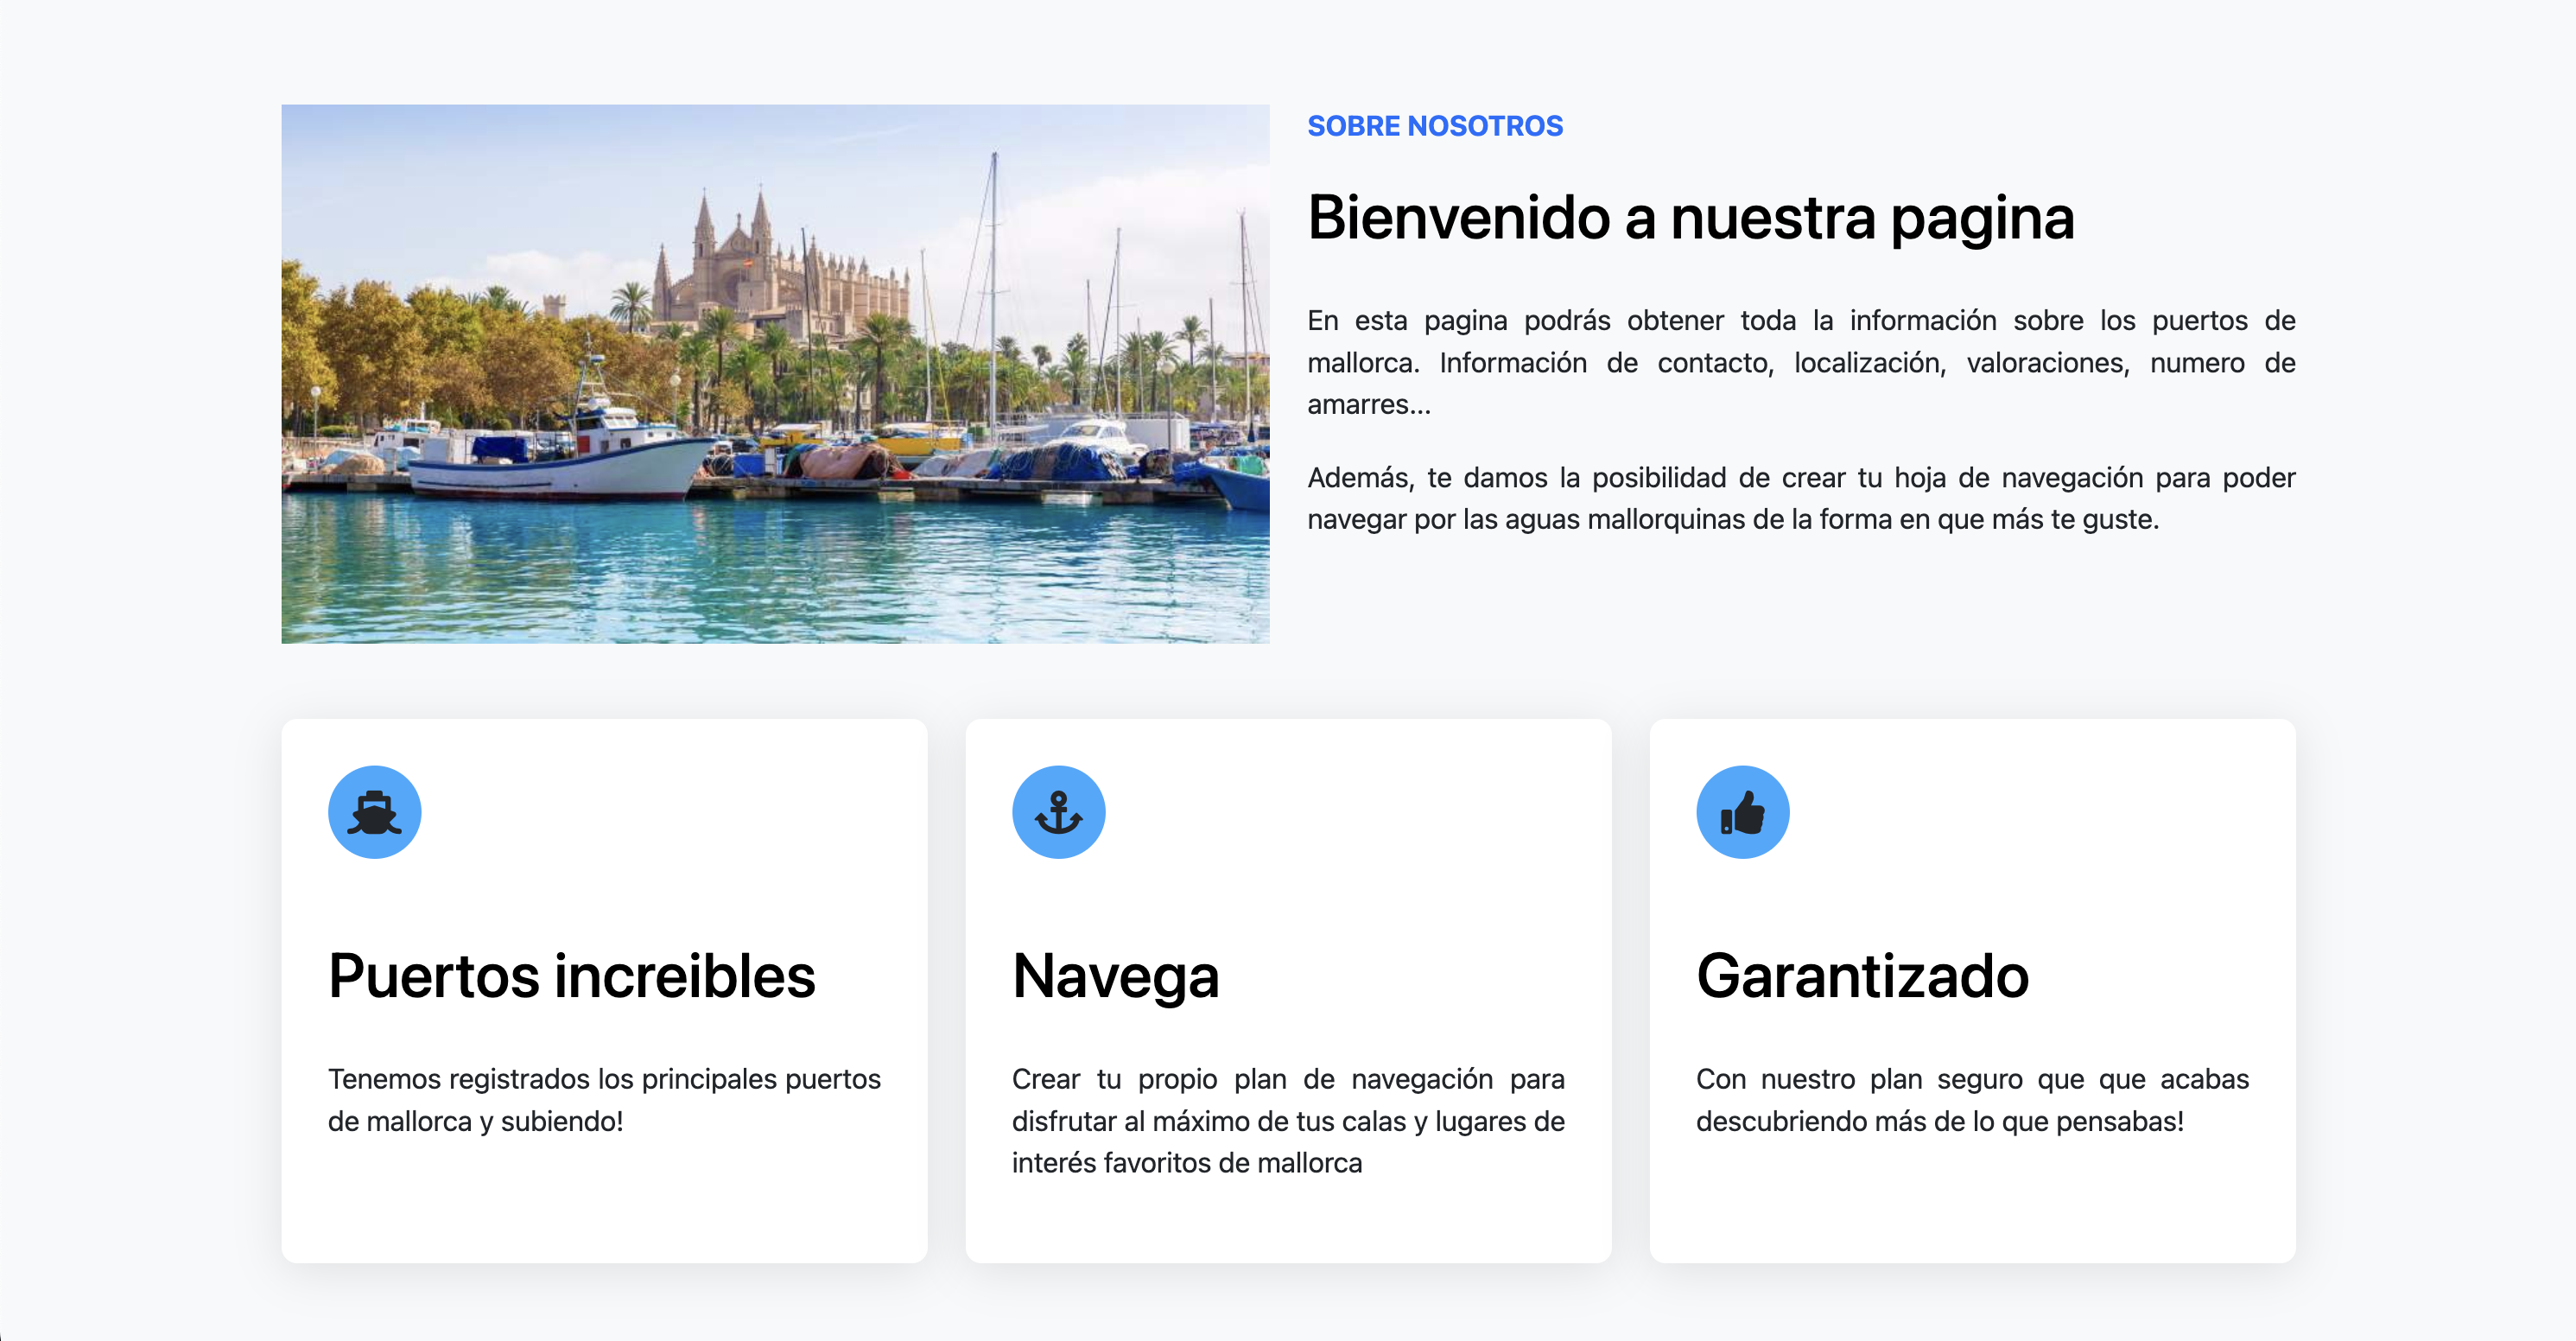
\includegraphics[width=0.7\textwidth]{images/introduccion.png}
    \caption{Sección introductoria de la web-app}
\end{figure}
\\Más abajo, encontramos la primera funcionalidad de nuestra web-app. Se muestra un mapa con marcadores rojos encima de los puertos registrados en la página. El mapa es interactivo, ya que se ha realizado mediante la API de Google Maps (la especificación técnica se explica más adelante en la documentación). Permite al usuario clicar encima de uno de los marcadores y así poder ver el nombre de este y, en caso de que el usuario quiera, tendrá un link que lo redirigirá a la página con la información del puerto seleccionado.
\begin{figure}[ht]
    \centering
    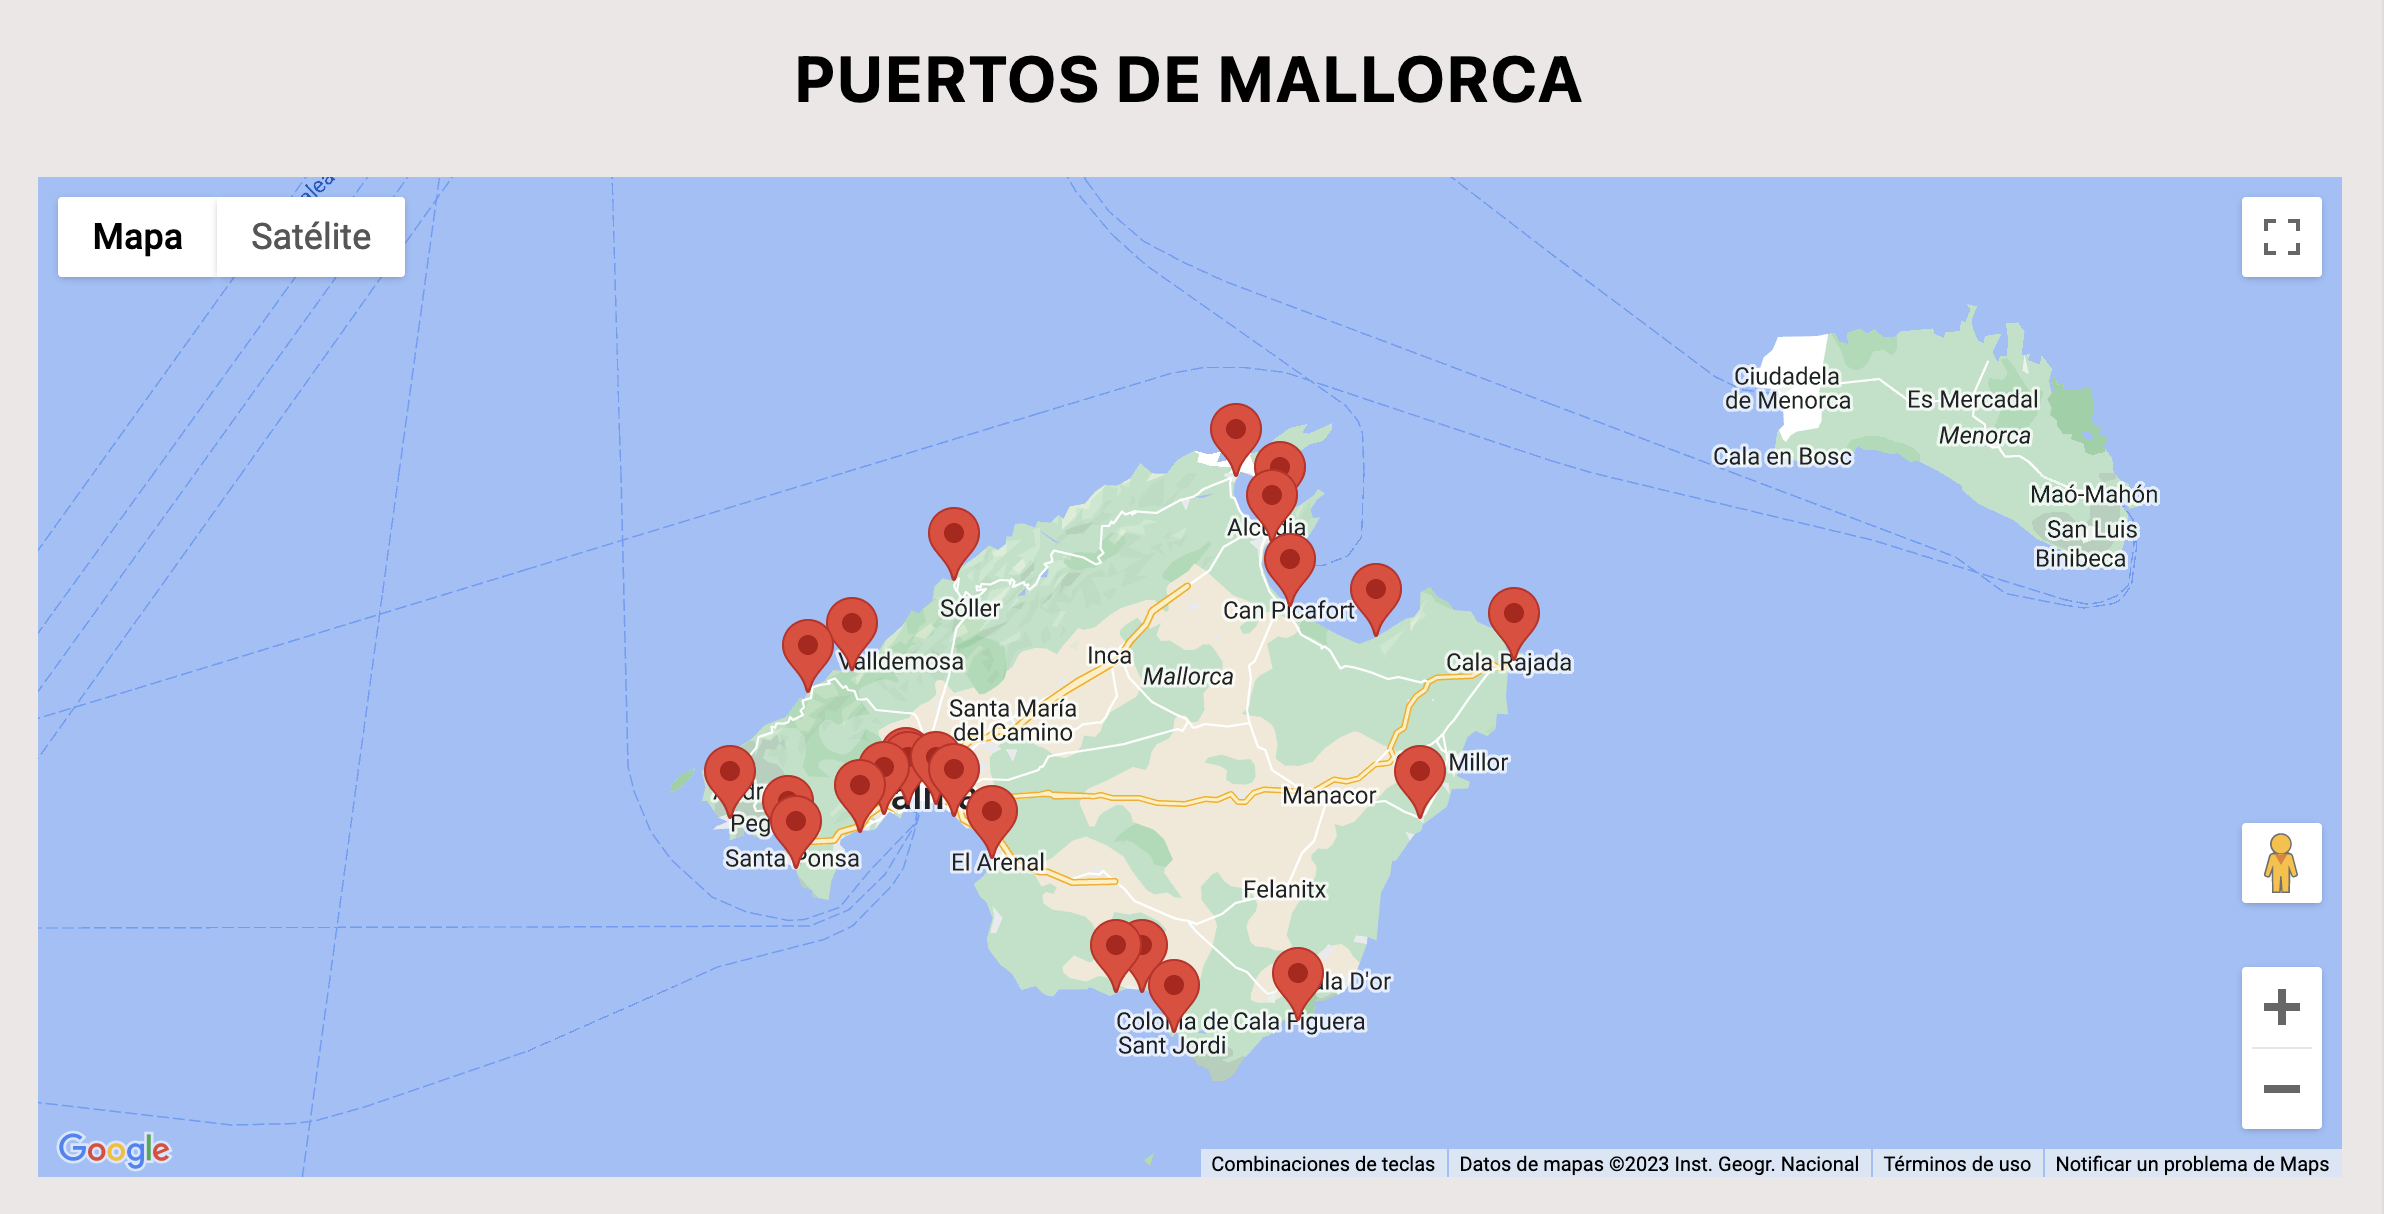
\includegraphics[width=0.9\textwidth]{images/mapa.png}
    \caption{Mapa interactivo de la web-app (actualmente solo hay dos puertos)}
\end{figure}
\\Debajo del mapa, encontramos otra funcionalidad de la web-app. Mediante la barra de filtros, podemos tanto filtrar los puertos por sus características como ordenar los puertos buscados por una de sus características. De esta forma, el usuario podrá buscar los puertos con mayor capacidad, los de mayor valoración o incluso saber los puertos con capacidad mínima de 300 barcos. 
\begin{figure}[ht]
    \centering
    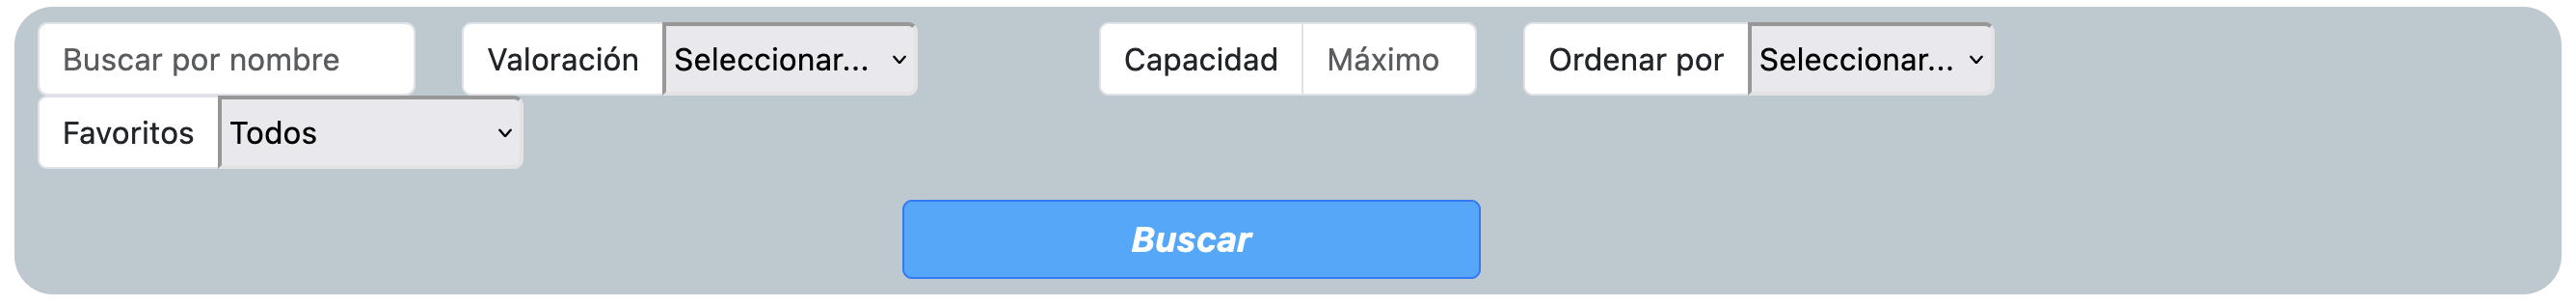
\includegraphics[width=1.0\textwidth]{images/filtros.png}
    \caption{Barra de filtros}
\end{figure}
\\Obviamente, la barra de filtros se aplica a las \texttt{cards} de los puertos que se muestran más abajo. En estas, se muestra su capacidad y su valoración en estrellas. También, si clicamos encima de la foto de uno de los puertos, nos redirigirá a la página del puerto en concreto.
\begin{figure}[ht]
    \centering
    \includegraphics[width=0.9\textwidth]{images/puertos.png}
    \caption{Ejemplos de \texttt{cards} donde se muestra una previsualización de los puertos}
\end{figure}
\\Para finalizar con la \textit{homepage}, encontramos el footer que encontramos en todas las sub páginas de nuestra web-app. En este, se muestran los nombres de los creadores de la página con sus respectivos links a sus páginas de GitHub, LinkedIn e Instagram.
\begin{figure}[ht]
    \centering
    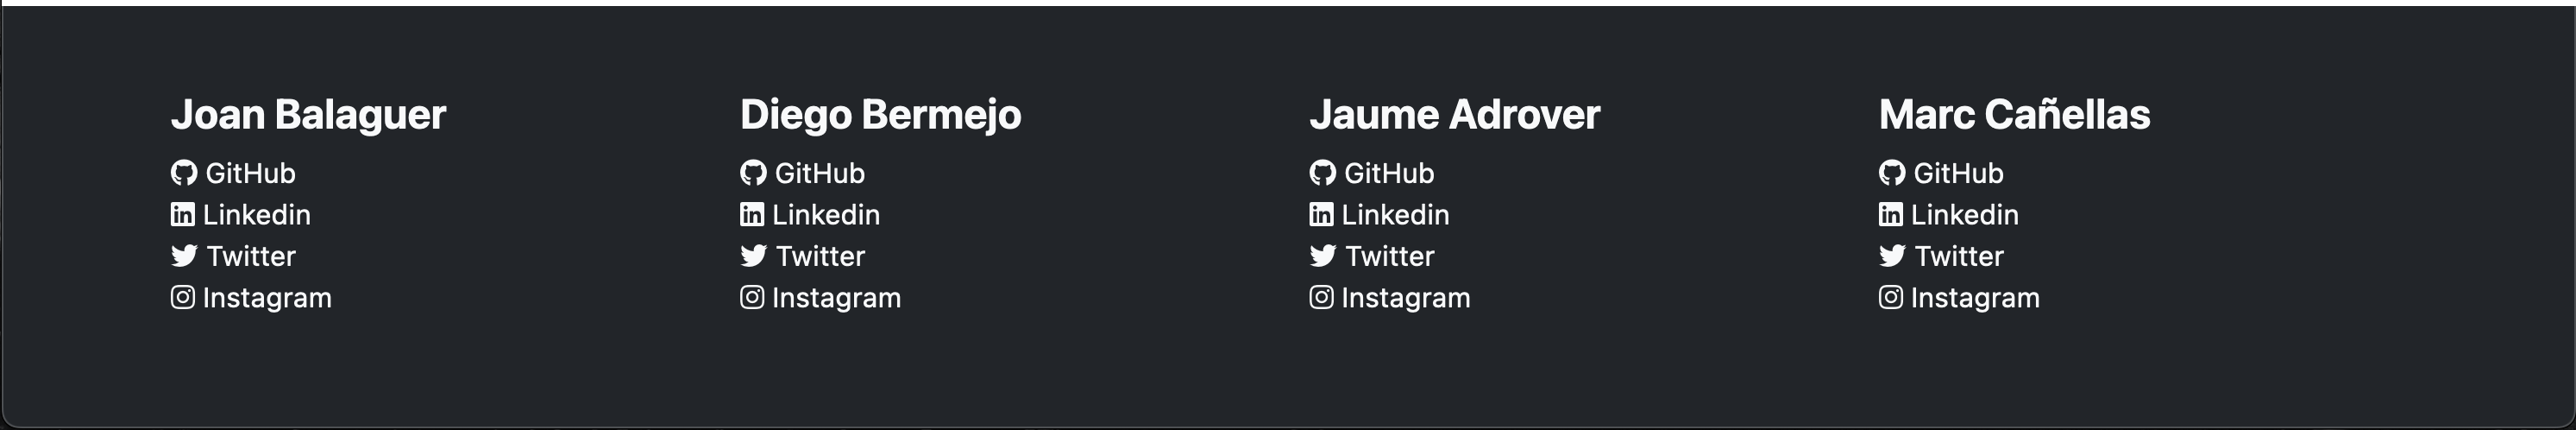
\includegraphics[width=0.9\textwidth]{images/footer.png}
    \caption{Footer de la web-app}
\end{figure}

\subsection{Página de un Puerto}
Cuando seleccionamos uno de los puertos, la web-app nos redirige a la página con información del puerto. Esta tiene diversas partes:
\begin{itemize}
    \item \textbf{Título}: simplemente muestra el nombre del puerto seleccionado en grande en la parte superior de la página.
    \item \textbf{Descripción y video}: muestra el atributo de la descripción del puerto, además del video que tiene también como atributo.
    \item \textbf{Características}: Muestra de forma concisa las características del puerto seleccionado. Se muestra su capacidad, su horario de apertura, si se permite fumar o no, la dirección, el correo electrónico, el teléfono y la valoración del puerto.
    \item \textbf{Tiempo}: en este apartado se mostrará el tiempo que hace actualmente en ese puerto en concreto.
    \item \textbf{Galería de Imágenes}: se muestran las imágenes que tenga como atributo el puerto seleccionado.
    \item \textbf{Lugares de interés cercanos}: sección en la cual se mostraran las playas, restaurantes y otros puertos cercanos.
\end{itemize}

\subsection{Plan de Navegación}

\subsection{Página de Contacto}

\section{Herramientas y Librerias}
Una vez se han explicado todas las funcionalidades que el usuario puede realizar en nuestra web-app, pasaremos a la explicación técnica de como se han implementado todas esas funcionalidades. Iremos revisando una por una las componentes de todas las páginas de la web-app y explicando que herramientas y librerías se han usado para su desarrollo.
\subsection{index.html}
El archivo \textit{index.html} contiene el código HTML de la \textit{homepage}. El contenido funcional de esta parte de la web-app ya se ha explicado a nivel de usuario, en esta sección se describirá como se han desarrollado esas funcionalidades a nivel técnico.

\subsubsection{Barra de Navegación}

\noindent Para la creación de la barra de navegación, se ha usado el framework \href{https://getbootstrap.com/}{Bootstrap}. Primero, hemos definido un objeto de la clase \texttt{container-fluid} el cual contendrá todo lo referente a la barra de navegación. Por otro lado, hemos añadido atributos a este contenedor para que el aspecto final de la barra de navegación sea el deseado:
\begin{itemize}
    \item \texttt{px-0}: elimina los márgenes horizontales (padding) del elemento, lo que significa que el contenido del elemento se extiende hasta los bordes laterales del contenedor.
    \item \texttt{d-flex}: define el elemento como un contenedor flexible, lo que significa que sus elementos hijos se pueden ajustar dinámicamente para adaptarse a diferentes tamaños de pantalla.
    \item \texttt{align-items-center}: alinea verticalmente los elementos hijos del contenedor, centrándolos en el eje vertical.
    \item \texttt{fixed-top}: fija el elemento en la parte superior de la pantalla, de modo que permanece en su posición incluso cuando el usuario se desplaza hacia abajo en la página.
\end{itemize}
Una vez sabemos como hemos definido el contendor, vamos con los elementos que se encuentran dentro de este. El principal elemento es un objeto de la clase \texttt{navbar navbar-expand-lg}. Esta, se utiliza para crear una barra de navegación responsiva en un sitio web (esto último es lo que indica el \texttt{expand-lg}). Dentro de esta, encontramos ya los botones que contienen la barra de navegación:
\begin{itemize}
    \item \textbf{Logo}: se ha realizado mediante la clase \texttt{navbar-brand}, perteneciente a Bootstrap. Dentro de este se encuentra la imagen del mismo.
    \item \textbf{Nombre de la página}: el nombre de "Puertos Mallorca" contenido en la barra de navegación, se encuentra dentro del objeto del logo. Este es otro objeto de la clase \texttt{navbar-brand}.
    \item \textbf{Botón de navegación}: este botón solo aparece en caso de que la pantalla donde se muestra la web-app no sea lo suficientemente grande como para mostrar todos los botones de la barra de navegación. En caso de suceder esto, aparecerá un botón con el cual podremos acceder a los botones que explicamos a continuación. Esto se ha hecho gracias a la clase \texttt{navbar-toggler} de Bootstrap. referenciando al objeto al que influye con el parámetro \texttt{aria-controls}. Mediante este, indicamos que el objeto con \texttt{id = navbarSupportedContent} se le aplicará la contracción de los botones cuando la pantalla no se alo suficientemente grande.
    \item \textbf{Botones de funcionalidades}: los botones de "Ver Puertos", "Plan de Navegación" y "Contacto" son objetos del tipo \texttt{nav-item} (items de una barra de navegación) de boostrap y están contenidos dentro de un objeto \texttt{collapse navbar-collapse}. Este objeto permite la contracción de los botones que hemos explicado en el apartado anterior.
\end{itemize}

\subsubsection{Carousel}
El deslizable con fotografias de los puertos, se ha realizado cogiendo como base la tercera de las \href{https://getbootstrap.com/docs/5.3/components/carousel/}{plantillas} que proporciona la página de boostrap para hacer estos carousels. Partiendo de esa base, nosostros hemos añadido las captions y la flecha que permite al ususario ir más abajo de la página. Las captions se crean con ojectos de la clase \texttt{carousel-caption} y los botones para ir más abajo de la página, son objetos de la classe \texttt{btn btn-down} de boostrap. Estos nos permiten crear un boton con forma de flecha como la que aparece en la web-app y mediante un \texttt{href} en su interior, linkeado con la parte inroductoria de la página, hacemos que cuando cliquemos encima de este nos lleve más abajo.

\subsubsection{Sección introductoria}
Este apartado contiene dos secciones principales: una sección de introducción con una imagen y un texto descriptivo, y una sección de tres columnas con información destacada sobre los puertos de Mallorca.\\

\noindent En la sección de introducción, hemos hecho un contenedor de HTML div con la clase \texttt{site-section} y un identificador \texttt{intro}. Dentro de este contenedor, hay otro contenedor de \texttt{div} con la clase \textit{container} y un contenedor de fila de div con la clase \texttt{row}. Esta fila contiene dos columnas de div con las clases \texttt{col-md-6} de Bootstrap. En la primera columna, hay una imagen con la clase \texttt{img-fluid}. En la segunda columna, hay un título con la clase \texttt{text-black} y un subtítulo con la clase \texttt{text-primary}.\\

\noindent En la sección de tres columnas, encontramos un contenedor de div con la clase \texttt{py-5}, un contenedor de div con la clase \texttt{container} y un contenedor de fila de div con la clase \texttt{row}. Dentro de esta fila, hay tres columnas de div con las clases \texttt{col-md-6 col-lg-4} también de boostrap. Cada columna contiene un contenedor de div con la clase "puertosIncreibles" (clase que luego usamos para referencial algunos objetos en css) que contiene un icono en un contenedor de \textit{span} con la clase \textit{circulo} y un título de ancla con la clase \texttt{tituloIntroduccion}. En resumen, esta sección presenta una breve introducción a la página y destaca tres características principales de la web relacionadas con los puertos de Mallorca.\\

\noindent Para la creación de esta sección introductoria, nos hemos inspirado en una sección similar que encontramos en \href{https://themewagon.github.io/waterboat/}{esta plantilla}.

\subsubsection{Mapa de puertos}
Para la creación del mapa, hemos usado la API que proporciona Google de su servicio Google Maps. Con \href{https://developers.google.com/maps?hl=es%2F%3Fq%3Dapis%20google}{esta}, podemos mostrar un mapa de google maps interactivo, ademas de los marcadores de los puertos que tenemos registrados en la pagina.

\noindent El mapa se encuentra contenido dentro de un objeto de la clase \texttt{container-fluid} de Bootstrap. Dentro de este, hemos añadido el div correspondiente al mapa, el cual le hemos añadido el identificador \texttt{map}. En cuanto al HTML, esto sería todo lo que necesitamos para crear el mapa. Siguiendo la documentación que proporciona Google sobre como crear los mapas, hemos implementado el fichero de JavaScript adjuntado en el proyecto llamado \textit{mapa.js}. Este contiene las instrucciones necesarias para la creación del mapa en la web-app. \textbf{(Actualmente, el script simplemente inicializa el mapa y crea dos marcadores de ejemplo. En la versión final de la documentación mostraremos como creamos dinámicamente según la información contenida en el fichero JSON de puertos, los diferentes marcadores y explicaremos el código necesario para inicializar el mapa)}

\subsubsection{Barra de filtros}
Para la barra de filtros y ordenación, también hemos usado el framework Bootstrap. Por tanto, todas las clases que se usan para los elementos de la barra de filtros son pertenecientes a este.\\

\noindent Toda la barra de filtros está contenida dentro de un elemento de la clase \texttt{container-fluid} para hacer que el contenedor ocupe todo el ancho de la pantalla. Dentro de este contenedor, hay un elemento \texttt{row} con la clase \texttt{filterSearch} y \texttt{align-items-center}, lo que indica que se trata de una fila que contiene elementos centrados verticalmente. Además, hemos utilizado la clase \texttt{py-2} para agregar un espacio vertical a la fila. Dentro de la fila, hay cuatro columnas definidas usando la clase \texttt{col-xs-12 col-sm-6 col-md-3}. Estas columnas son para los elementos de búsqueda por nombre, valoración, capacidad y ordenar por. Dentro de cada columna, se utiliza la clase \texttt{input-group} para agregar estilos a los elementos de entrada de texto y select. Cada uno de estos elementos tiene una etiqueta de texto que describe la entrada que se espera.\\

\noindent El botón de búsqueda está dentro de una columna de 12 columnas y utiliza la clase \texttt{d-flex justify-content-center} para centrarlo horizontalmente. Se le da un identificador \texttt{botoCerca} (que usaremos posteriormente en los scripts de javascript) y se le asigna la clase \texttt{btn btn-primary mt-3} para darle un estilo de botón. Además, se utiliza la función \texttt{PortSearch()} \textbf{(actualmente no está desarrollada esta función, pero será la encargada de que se muestren unos puertos u otros en la siguiente sección de la web-app)} cuando se hace clic en el botón.

\subsubsection{Cards de puertos}
Justo debajo de la barra de filtros, encontramos los puertos que podemos filtrar i ordenar mediante esta. Esta sección se encuentra encapsulada en un \texttt{container-fluid} de Bootstrap, de los cuales ya hemos hablado en esta documentación. Dentro de este contenedor, encontramos varias filas de objetos de la clase \texttt{card}. Las filas las definimos mediante la clase \texttt{row equal-width} y las columnas de estas filas con la clase \texttt{col-md-3}.\\

\noindent Por lo que respecta a los recuadros de los puertos, el framework de Bootstrap tiene una clase llamada \href{https://getbootstrap.com/docs/5.3/components/card/}{Card}, con la cual puedes crear recuadros con una foto y una pequeña sección de texto. Este tipo de objetos son los que hemos elegido para mostrar una previsualización de los puertos registrados en la página. \textbf{(Actualmente, en los objetos de clase \textit{Card} están definidos de forma estática. la idea es que se creen dinámicamente estas cards mediante la información del JSON y se muestren unos puertos u otros en función de los filtros y criterios de ordenación que haya seleccionado el usuario en la barra de filtros)}.\\

\noindent La estructura que siguen todas las \texttt{cards} es la siguiente:
\begin{itemize}
    \item El primer elemento es una etiqueta \texttt{a} que envuelve una imagen (\texttt{img}) y que sirve como enlace a la página del puerto al que pertenezca la \texttt{card}. Mediante este enlace, el usuario podrá navegar y ver la información de diferentes puertos.
    \item El segundo elemento es un \texttt{div} con la clase \texttt{card-body} que contiene el contenido principal de la card. Dentro de este, mostraremos la información textual del puerto (nombre, capacidad y valoración).
    \item Dentro del div con la clase \texttt{card-body}, hay un elemento h5 con la clase \texttt{card-title} que muestra el título de la card (en este caso será el nombre del puerto).
    \item También hay una lista no ordenada (\texttt{ul}) con un solo elemento (\texttt{li}) que muestra la capacidad del puerto.
    \item Finalmente, hay un \texttt{div} con la clase rating que contiene estrellas de valoración de la clase \texttt{fa fa-star} y un párrafo (\texttt{p}) que muestra la valoración promedio del puerto.
\end{itemize}

\subsubsection{Footer}
Finalmente, en la \textit{homepage} encontramos el footer. Esta sección comienza con una etiqueta \texttt{<footer>} que tiene una clase \texttt{bg-dark text-light py-5}, lo que significa que el fondo del pie de página será oscuro y el texto será claro. Además, el padding superior e inferior de la sección será de 5 píxeles.\\

\noindent Dentro del pie de página hay un contenedor de la clase \texttt{container} que contiene una fila (\texttt{row}) con cuatro columnas (\texttt{col-md-3 mb-4 mb-md-0}), cada una con información de un miembro del equipo.\\

\noindent Cada columna comienza con un encabezado (\texttt{fw-bold mb-2}) que muestra el nombre del miembro del equipo y luego se muestran tres iconos que representan los enlaces a los perfiles de cada miembro en Github, Linkedin e Instagram respectivamente. Los enlaces se abren en una nueva ventana (\texttt{target="\_blank"}) y no se les permite la seguridad adicional de referencias (\texttt{rel="noopener noreferrer"}).

\subsection{puerto.html}
En este fichero HTML está contenido las estructuras para poder mostrar al usuario la información sobre un puerto en concreto. En las explicaciones siguientes, se obvian la barra de navegación y el footer (ya explicados en la \textit{homepage}).

\subsubsection{Nombre del puerto}
El nombre del puerto simplemente de trata de un contenedor con un \texttt{h1} que muestra bien en grande como se llama el puerto seleccionado. Además, mediante \textit{CSS} se ha añadido una imagen de fondo para dar un ambiente más marino.

\subsubsection{Descripción y Video}
En esta sección de la página, se muestra la descripción del puerto seleccionado, además de un video que lo muestra. Ambas cosas son atributos que obtenemos del fichero JSON de puertos.\\

\noindent Los dos atributos se encuentran en un objeto \texttt{container-fluid} y dentro de este mostramos una fila con dos columnas. Cada una de ellas es uno de los atributos. La descripción está contenida en una columna de la clase \texttt{col-md-8 col-lg-6} y el video en una columna de clase \texttt{col-md-4 col-lg-6 mb-4 align-self-center}. El video se encuentra en un \texttt{div} de clase \texttt{embed-responsive embed-responsive-16by9 custom-embed-responsive}, que nos permite poner un video de YouTube justo al lado de la descripción del puerto, de forma que este se pueda reproducir sin necesidad de abrir una pestaña nueva con el link del video.

\subsubsection{Características}
\textbf{Aun no desarrollado}
\subsubsection{Tiempo}
\textbf{Aun no desarrollado}
\subsubsection{Galería de Imagenes}
\textbf{Aun no desarrollado}
\subsubsection{Lugares de interés cercanos}
\textbf{Aun no desarrollado}

\subsection{navegate.html}
\textbf{Pagina aun no desarrollada}

\subsection{contact.html}
\textbf{Aun no desarrollado}
\section{APIs utilizadas}
\subsection{OpenWeatherAPI}
\subsection{EmailJS}
\subsection{Youtube}
\end{document}